\documentclass[a4paper]{article}

%% Language and font encodings
\usepackage[english]{babel}
\usepackage[utf8x]{inputenc}
\usepackage[T1]{fontenc}

%% Sets page size and margins
\usepackage[a4paper,top=3cm,bottom=2cm,left=3cm,right=3cm,marginparwidth=1.75cm]{geometry}

%% Useful packages
\usepackage{amsmath}
\usepackage{graphicx}
\graphicspath{ {images/} }

\usepackage[colorlinks=true, allcolors=blue]{hyperref}

\title{Assignment 6 - First Implementation of your System (FIS)}
\author{ by Group 3 - Plant-Id \\* \\* Team Members: \\* Ethan Ahuja - ahujae \\* Ethan Patterson - patteret \\* James Barry - barryj \\* Evan Brass - brassev \\* \\* Customers: \\* Ethan Ahuja - ahujae \\* Ethan Patterson - patteret}
\begin{document}
\maketitle
\pagebreak
\tableofcontents
\pagebreak
\section{GitHub Link}
As requested in the assignment description, the GitHub branch for this assignment can be found here: \url{https://github.com/barryjosu/CS361-001-W2018/tree/plant-id-assignment-6}

\section{Product Release}
Since we are developing an Android application, we are working to make it available for free on the Google Play Store. However, the app can currently only be run by building it with Android Studio and running it on an Android phone or Android emulator (built-in in Android Studio). Note that the current prototype was developed for Android version 21, so past versions will very likely not be able to run it. However, versions beyond 21 should be able to run it. We have a GitHub repository we are using to collaborate, and more detailed install instructions can be found there: \\*
\url{https://github.com/boxman888/Plant-Id-Android}
\pagebreak
\section{User Stories}
\subsection{Story 5}
\begin{center}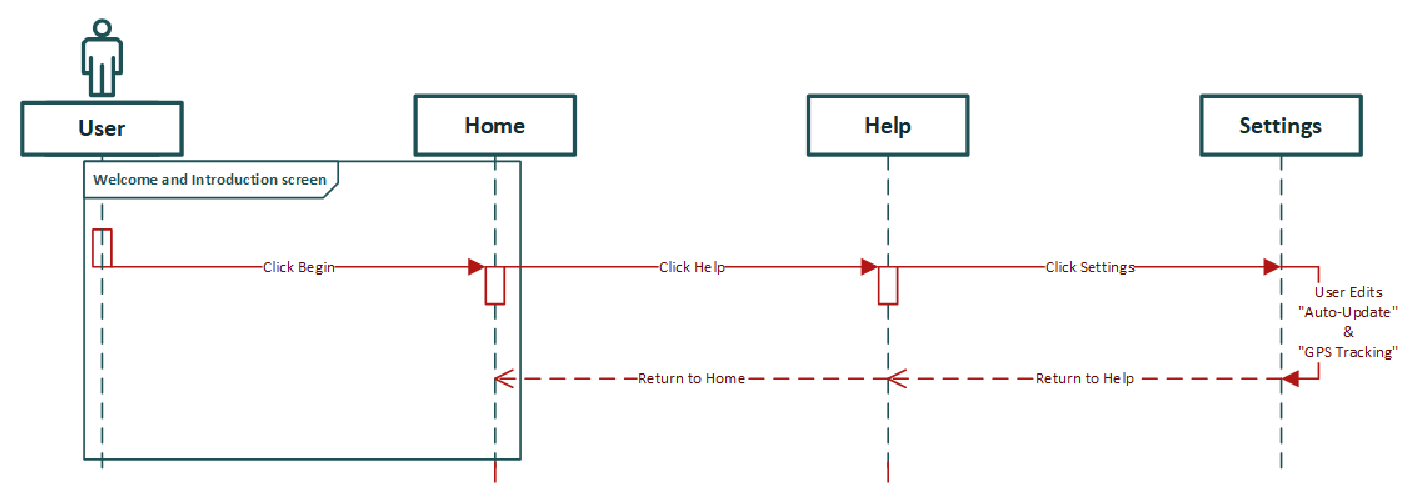
\includegraphics[scale=.66]{Story5.eps}\end{center}
This story was implemented by Ethan A and Ethan P during our 3/3/2018 meeting, and was finished by Ethan A, Ethan P, and James B during our 3/5/2018 meeting. It is the settings page for the application. We are learning how to use Android Studio as we go, which has been a large development hurdle. This story in particular gave us issues because of what seemed to be a bug with the studio. It has a built-in tool for generating a settings page that saves preferences, but the option failed to generate some of the support files needed and caused us a lot of confusion. It created some references in pre-existing XML files in order to integrate the settings page, but since those support files failed to generate, we had to figure out where these XML edits were made so we could revert them. The fact that Android Studio auto-saves made this needlessly difficult. 

This story took about three hours to implement due to these issues. It is implemented and has been simplistically tested. No automated test cases were built, but the simply functionality appears to be working fine. The diagram that we developed for this story was good for reference, but didn't feel terribly important because of how simple this story is. It could have been described adequately with a few sentences. There is no work left for this story, aside from cosmetic changes.
\subsection{Story 6}
\begin{center}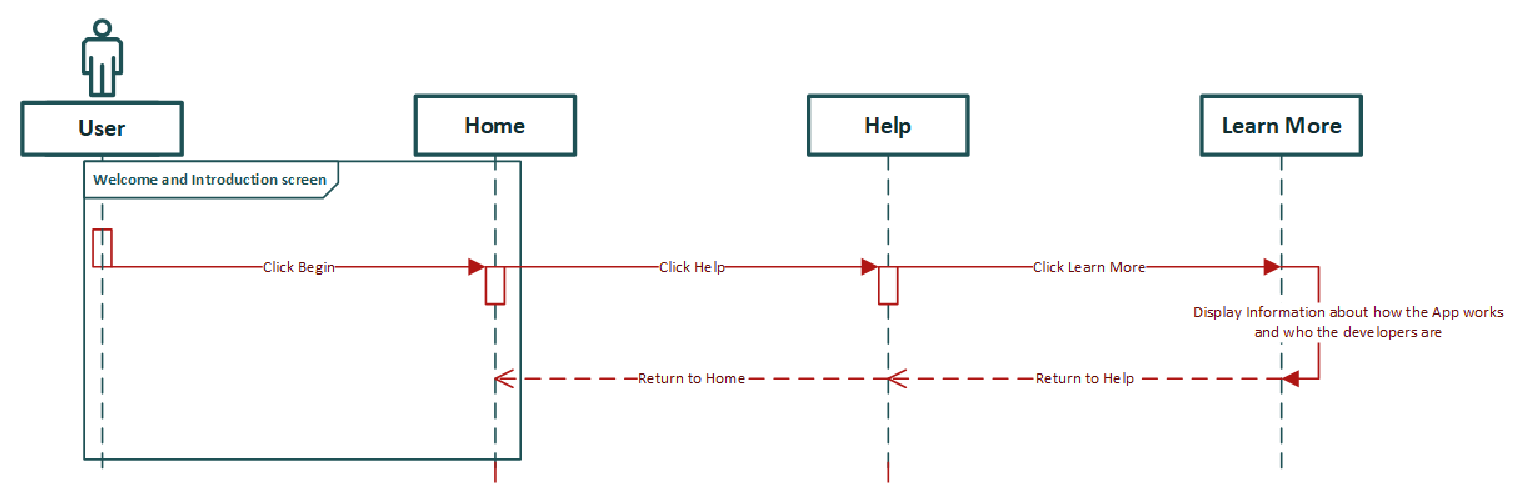
\includegraphics[scale=.66]{Story6.eps}\end{center}
This story was implemented by Ethan A and Ethan P during our 3/3/2018 meeting. It is for displaying an "about the app" page to the user. Due to the simplicity, we ran into no difficulties beyond our inexperience with Android Studio. It took about an hour to implement and verify that it was functioning properly. The UML diagram for this story didn't feel very needed, since the story was so simple. The story has been tested thoroughly, although without any automated testing, and there is nothing left to implement for it. 
\pagebreak
\subsection{Story 7}
\begin{center}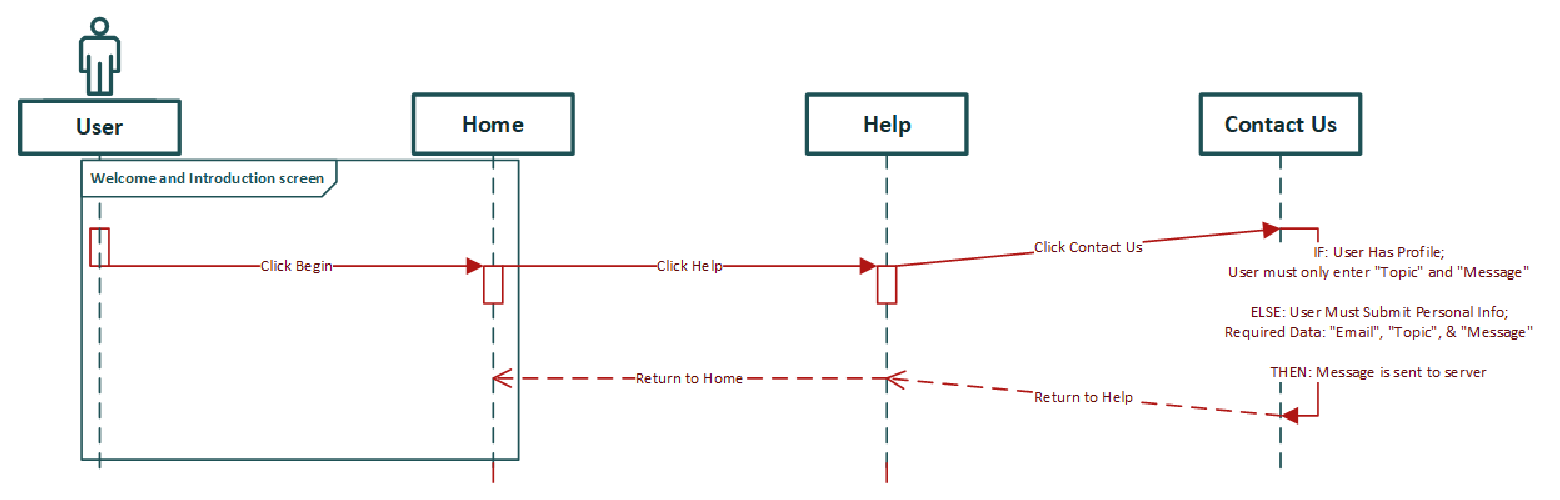
\includegraphics[scale=.66]{Story7.eps}\end{center}
This story was a bit more complicated than the others, since it required actually sending information up to our database. It was implemented by Ethan A, Ethan P, and James B during our 3/5/2018 meeting. It is for sending feedback to the application developers. We didn't run into any difficulties during implementation, though, so it only took about an hour to implement. We verified that it was functioning properly, but have not done very thorough testing to ensure that no bad values get through to the database. The UML diagram was quite helpful for this, although we are not supporting the account-related functionality described in it because we have decided to drop account support.
\subsection{Story 10}
\begin{center}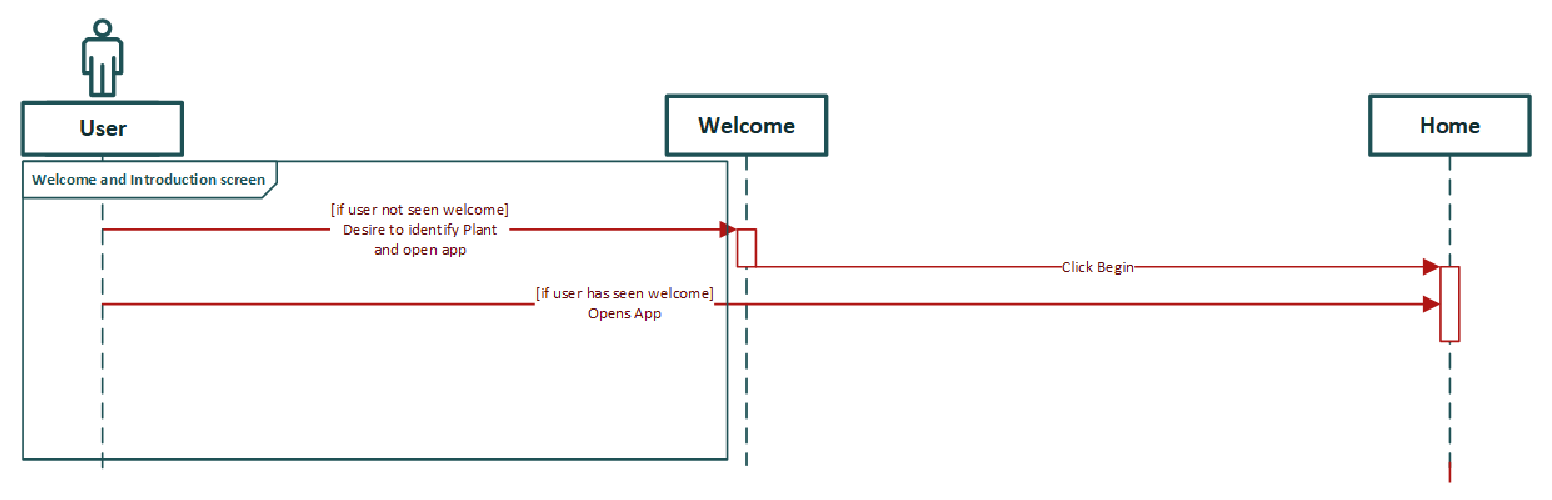
\includegraphics[scale=.66]{Story10.eps}\end{center}
This story was implemented by Ethan A and Ethan P during our 3/3/2018 meeting. It is a welcome page that displays when the app is first opened. We changed our design for this a bit, opting to instead display the welcome page every time the app is opened. As a result, the UML diagram is not entirely accurate. It took about an hour to implement and we encountered no issues. No further changes are needed.
\pagebreak
\section{Design Changes and Rationale}
We were able to work directly with our customers during this part of the implementation, so we did not have to ask them any questions or make any major design changes. However, we have discussed abandoning some of the user stories that we outlined in our last assignment. The original idea behind these user stories is that they would be implemented if time allowed, but the busy schedules of our team are making it very clear that these stories will need to be dropped. These stories include: 
\begin{itemize}
\item Story 2: Image Identification - A neural network that would identify plants based on an image supplied by the user. This is too large of an ordeal to implement within our time constraints.
\item Story 8: Create an Account - Users could make an account on the application to save a history of plants they have identified. There are a few auxiliary stories for this one. This would not be too complex to implement on its own, but wouldn't serve much purpose without also implementing the auxiliary stories.
\item Story 9: Become a Botanist - An auxiliary story for story 8. Professional botanists could become certified botanist users through a verification process, allowing them to review geotag information in the database. This poses security risks, and our team is also not familiar with how to verify if someone is a professional botanist. 
\item Story 11: Reward System - An auxiliary story for story 8. Users would be able to receive in-app achievements by fulfilling certain goals, giving them Google Play Store points. 
\item Story 12: Social Media - Users would be able to connect a social media account (FaceBook, Twitter, etc) with their Plant-Id account to share their findings online. 
\end{itemize}
We will be moving forward with the following stories as originally outlined: 
\begin{itemize}
\item Story 1: 20 Questions - We implemented part of this story this week, as outlined above.
\item Story 3 and 4: Incorrect and Correct Identification - Once 20 questions is implemented, we will implement displaying information relevant to the identified plant once the app thinks it has identified something. Then, the user will be able to provide feedback if they think the identification is wrong.
\end{itemize}
We did wish that we had had a UML diagram for story 1, since we implemented some of the basic features of that, but were able to communicate everything needed with our customers since we were working directly with them.

\pagebreak
\section{Tests}
It's a bit early for us to be designing test cases, but we've designed a few simple ones to ensure our limited features work properly. Some of them are not automated, since we'd like to ensure that the application works properly when a user is interacting with it in real time. Some of our stories also can't really be verified automatically. At this stage, we are mostly focusing on ensuring that our activities (Android IDE terminology for pages/views in the application) display their intended information. 
\subsection{Major Component Unit Tests}
We outlined some unit tests on paper for the components we implemented this week. Since these stories are basically all related to navigating around the app, we simply tested out all the buttons in order on a few different Android environments. The new buttons we implemented this week include Settings, Learn More, and Contact Us. We chose to not automate these tests because there's no logical way to automatically verify the output of these cases, since it's simply ensuring that the activities in the application look correct.

Our unit test plan was to simply install the application, open it, ensure the welcome page was displayed, and then navigate to these new buttons. This means start by clicking on the Help button. Then, click on the Settings button and ensure both options can be toggled between "yes" and "no." Then, click the "back" arrow to get back to the Help page and click on Learn More. Review the information displayed and ensure it looks as intended. Finally, click the "back" arrow again and then go to the Contact Us page. Enter some information in the box and send it. Then, check the database to ensure that the information sent through properly. We focused on a few cases for this to ensure no bad values can get through, namely trying to send an empty string. We escape out the input, so no database commands can be sent this way to potentially sabotage the database.
\subsection{Major User Story Unit Tests}
On our back end, we started working on a simplistic implementation of the 20 Questions story. It's not currently present in the actual application, since we have not built any interface for it. However, we were able to use Maven with JUnit to do some simple automated testing. We gave a series of "yes" and "no" inputs and asserted that the result question or name of the result plant was correct. Here's an example of two of our tests. 
\begin{center}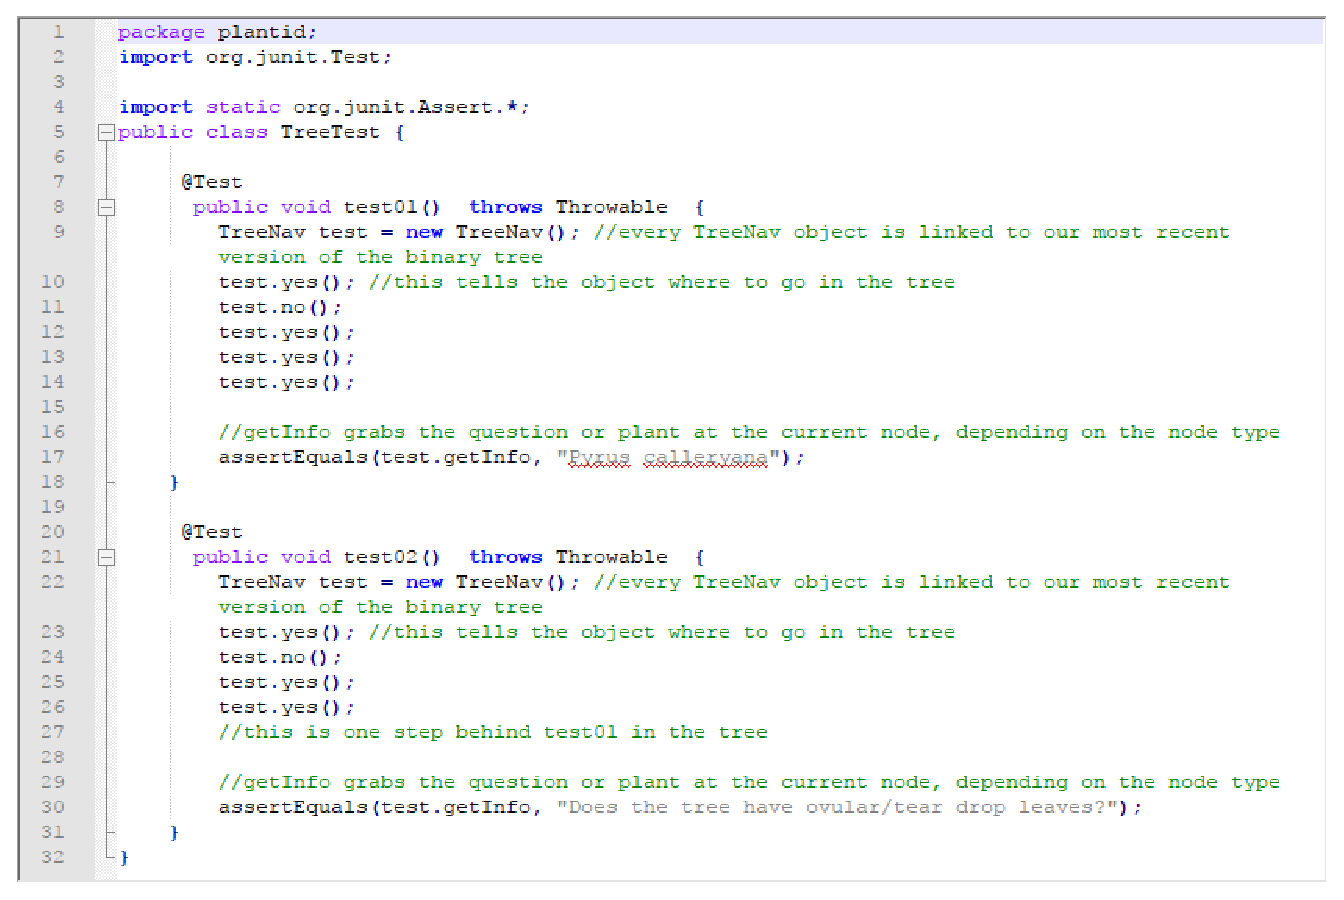
\includegraphics[scale=.66]{test.eps}\end{center}
As the comments explain, these tests navigate to a position in the tree and then verify that the information there is as intended. Note that these tests will become obsolete as we expand our tree, since the location of the tested plant and question will likely change. We will likely follow a similar structure for testing in the future.
\subsection{Further Unit Tests}
Once we have developed an interface for the 20 questions implementation, we hope to automate testing in a new way. We can use Ranorex or Sikuli with our Android IDE to develop tests that automate input within the Android app itself. Ranorex does it by assigning IDs to buttons in the app, allowing test cases to be built out of inputting these IDs. Sikuli does it by allowing test cases to make inputs at specified locations on the virtual screen using coordinates. This will allow us to escape doing backend testing and instead test in a real-time environment. We still won't be able to do automated testing on an actual device, since these libraries are only compatible with Android emulators, but we can still do some manual verification on an actual device to ensure that the outputs match the results from the emulator.

These new tests will still require some user interaction, since there's no effective way to verify output at the end of a test, but the interaction will be minimal. The tester will simply have to look at the screen and ensure everything is in order. We can create a list of what we expect each test to output so that the tester knows what to look for. The structure for these tests will be similar to the backend tests described in section 5.2, giving the application a series of "yes" and "no" button presses and then verifying that the resulting plant or question matches what is expected.

The only aspects of our program that require internet connection are the option to leave feedback for the developers and report incorrectly identified plants. We'd like to focus on these cases next week so we can verify that we are properly handling any connection errors. We don't currently deal with issues like terminated connection or trying to send feedback without a connection. 

We would also like to try testing the application more on various environments, since ensuring platform compatibility is a big part of Android testing. We'll focus in on this during quality testing, after we've implemented all our required features for the application. We will try running the application and our unit tests on various different Android versions, such as 26, 27, and 28, as well as the 32-bit and 64-bit versions of them, and running our unit tests on each version too. Note that Android applications cannot be run on versions older than the version they were developed for, so we don't need to worry about versions older than 21. 

There are also other aspects of testing we'd like to consider later on. Some obvious ones include battery consumption, data requirements, and application speed. Ideally we can balance speed, accuracy, and efficiency, and it should be fairly easy to achieve given the simplicity of our application. However, we would like to view its hardware impact under various Android environments to ensure there's no major memory leaks causing lag or unnecessary battery usage. 
\pagebreak
\section{Meeting Report}
\textbf{03/03/2018 (12:00pm - 6:00pm):} Johnson Hall - Room 219
\begin{itemize}
\item Ethan A and Ethan P did paired programming to implement the user stories for this week.
\item James Barry joined the meeting remotely over Discord and did the documentation and unit test design.
\item As covered earlier in the document, we plan to finish implementing 20 questions and the stories for correct and incorrect identification by next week. The week after that will be spent cleaning up interface design and doing quality testing. 
\item Our customers met and participated and were reasonable with their requirements for the team.
\end{itemize}
\textbf{03/05/2018 (5:00pm - 7:00pm):} Johnson Hall - Room 219
\begin{itemize}
\item Ethan A, Ethan P, and James B did paired programming to implement the user stories for this week.
\item We finished implementation and cleaned up a few things on all user stories. Our next meeting will still be focused on implementing 20 questions. 
\item Our customers met and participated and were reasonable with their requirements for the team.
\end{itemize}
\end{document}
